\chapter{Concepts and Technologies}
\label{cha:concepts}

\section{Front-end}
\label{cha:concepts:sec:frontend}

\subsection{Typescript}
`` A super-set of JavaScript that compiles to plain JavaScript ''\cite{tswebsite}, Typescript is a language maintained by Microsoft and developed by \textit{Anders Hejlsberg} in 2012 with the goal of improving the quality and manageability of JavaScript code bases with features such as static typing and object-orientated qualities\cite{tsrevealed}. Ultimately, Typescript must be compiled to JavaScript before being executed, for compatibility reasons, the default JavaScript target is version ES3 but newer back-ends are also available.

\subsection{HTML}
The \gls{HTML}, the `` World Wide Web's core markup language ''\cite{html} is a declarative language through which the vast majority of online content is structured, shared and accessed. It is a specification of elements that can be used to structure the content of web pages, such as headings, images, link to other documents, buttons and many others\cite{htmlcss}.

\subsection{CSS}
\gls{CSS} is another declarative language that pairs with HTML. It's purpose is to describe how the elements present in a web page are presented.
Some of the definitions handle colors, fonts, element arranging, visibility, interaction and many others\cite{htmlcss}.

\subsection{SASS}
\gls{SASS} is a augmentation of CSS with features that are similar to a object-oriented languages, with loops, variables, functions and rule nesting \cite{sass}. SASS files need to be compiled into plain CSS before deployment, there are many of such compilers, some re-generate CSS files upon file  changes.

\subsection{Angular}
Front-end web framework developed as a side project at Google that proved itself as a valuable tool for modern application development. The core idea is that \gls{HTML} faults when it comes to declare dynamic content\cite{angularjs}, therefore a new middle-ware is introduced between the rendered page and the underling code so that all the elements and events in the \gls{HTML} document are captured and made available to it's components. Such binding goes both ways, so if the state of the underling code changes, the document is re-rendered to reflect the new state.

The first version of Angular is now called AngularJs and can be included in a \gls{HTML} document just like any other JavaScript library. This version proved it's value but was considered confusing and some times, slow. Since then it entered \gls{LTS} stage and no features are added. Angular version 2 and up is a Typescript re-write that includes some new features that aid in the architecture and development of scalable and reusable code, namely, the introduction of Components, Router, Ahead-of-Time compilation and Observables\cite{angular}.

\todo{Router}
\todo{Components}
\todo{Template}
\todo{angular cli}

\subsection{Angular Material}
Material Design is a set of guidelines and principles made by Google for designing \gls{UI} that aims to bring natural and consistent interactions between users and computers. The guiding principle is based on paper and ink but it is not limited to what they can do in the physical world\cite{materialdesign}.

Angular Material\cite{angularmaterial} is the implementation made by Google of components like buttons, text input and separators that follow the Material Design guidelines to be used by Angular applications, providing a consistent look across devices.

\subsection{Sb-Admin-Material}
To accelerate the development speed and have faster working prototypes, many web-based projects begin form a ready-made template. This saves time by keeping developers from re-writing common pieces of code commonly referred as ``boilerplate''.

SB Angular Material is a re-write of the famous SB Admin template\cite{angulartemplate}, a free and open source template developed by Start Bootstrap\cite{sbadmin} in Angular using components developed in the previously discussed Angular Material project.

As the name implies this template tries to assess the need for an administrator panel, and in doing so it provides a few ready-made components, to name a few, a login component as seen in figure \ref{fig:login}; the main screen with a top and a collapsible side navigation components, seen in figure \ref{fig:dash} and \ref{fig:visible}. This template already encompass some amount of responsive design by toggling the ability of said side navigational panel to be collapsed depending on the user's screen width.
% Ligatura com a proxima secao

\todo{ referenciamento da próxima secção, isso esta certo ?}

In the following subsection this template's folder structure will be explained so that one can understand where what are the main parts in which it can be extended to fit any particular project.

\begin{figure}
  \centering
  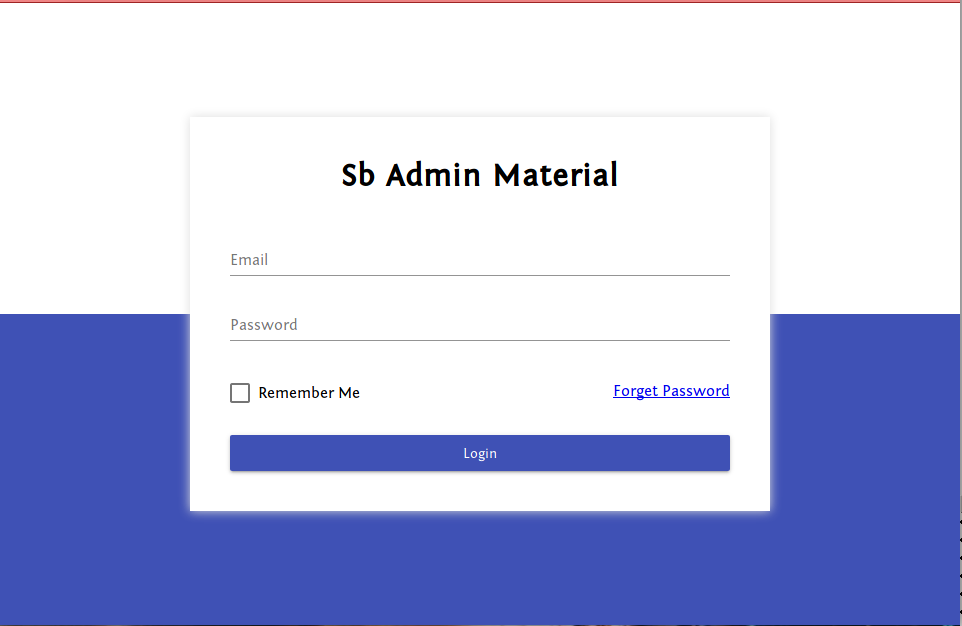
\includegraphics[width=.5\textwidth]{images/sbadmin/login}
  \caption{Login Screen}
  \label{fig:login}
\end{figure}
\begin{figure}
  \centering
  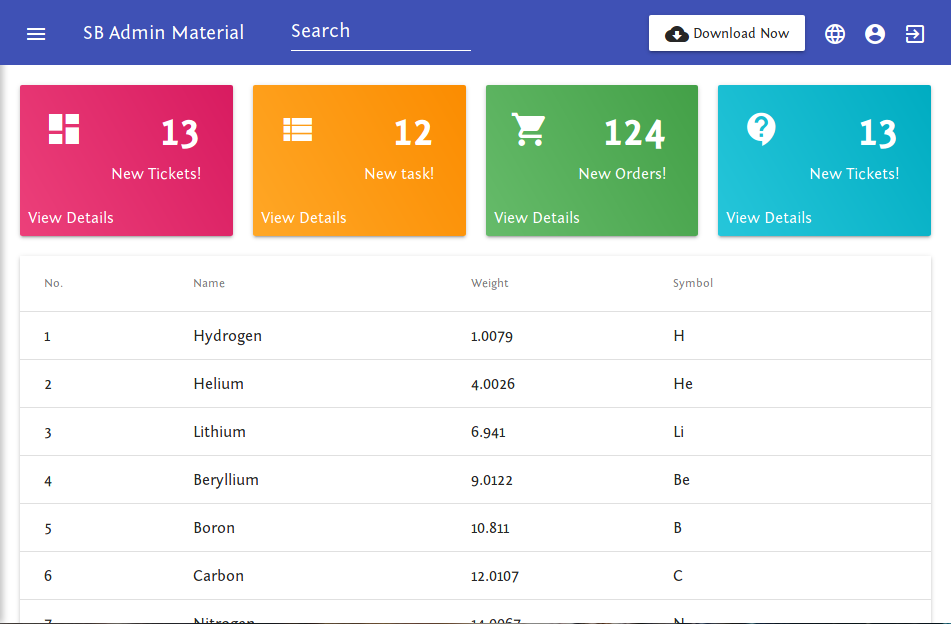
\includegraphics[width=.5\textwidth]{images/sbadmin/collapsed}
  \caption{Dashboard with collapsed side menu}
  \label{fig:dash}
\end{figure}
\begin{figure}
  \centering
  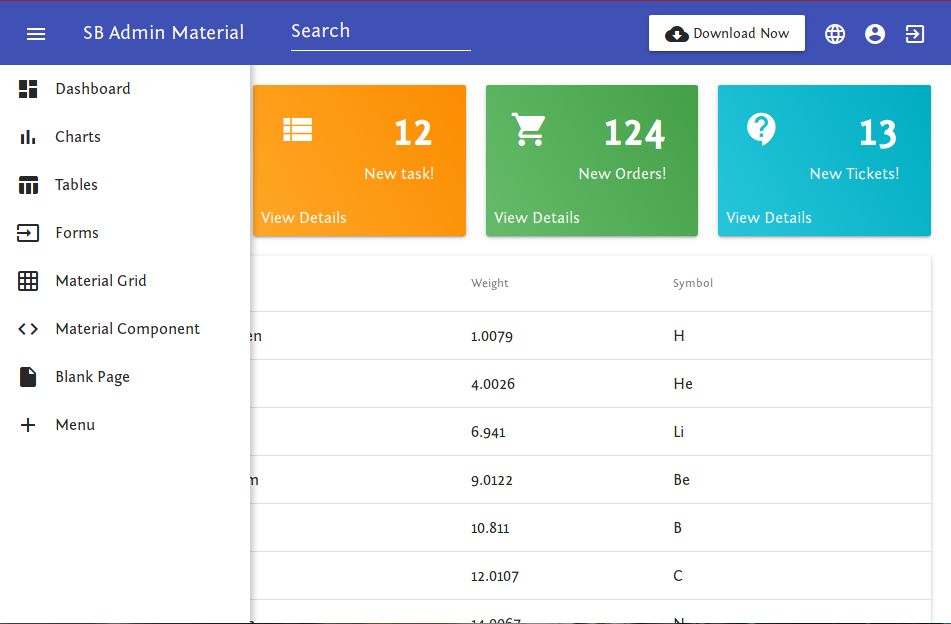
\includegraphics[width=.5\textwidth]{images/sbadmin/visible}
  \caption{Dashboard with visible side menu}
  \label{fig:visible}
\end{figure}

\subsubsection{Project Structure}
SB Admin Angular was written with the intention of being modified and extended by other developers. Because the team did not express any guidelines towards how it should be further developed, it is important to give an overview of the current project structure so that the changes made to accommodate the topic of this project are better understood.

\todo{ambientes descriptions aninhados ficaram bons ?}
\begin{description}
\item[root] This item is not a folder but the root of the project. In here there are configurations for code linter, JavaScript dependency descriptor and the license statement.
\item[dist] Once the project is built for deployment, this directory will hold all the assets and optimized code ready for production, including the main \texttt{index.html} file that bootstraps the whole project.
\item[e2e] This holds the source code for End-to-End test cases, hence the name.
\item[src] This is the heart of this template, a directory that holds all the structure, content and behavior needed per application. \leavevmode
  \begin{description}
  \item[app] The Angular entry-point and application wide router module. \leavevmode
    \begin{description}
    \item[layout] All the components used to compose the navigational elements and menus and their subsequent pages plus some example pages. \leavevmode
      \begin{description}
      \item[black-page] A inaccessible component that does nothing, probably unfinished.
      \item[blank-page] An example component that is white.
      \item[charts] A component that display chart capabilities of the integrated JavaScript module chartjs\footnote{Available at https://www.chartjs.org/}.
          \item[components] Omnipresent page elements such as the Topbar and the collapsible Sidebar.\leavevmode
        \begin{description}
        \item[topnav] The blue navigation top bar as seen on Figure \ref{fig:dash}.
        \item[sidebar] The Menu on the left side of the screen as seen on Figure \ref{fig:visible}.
        \end{description}
      \item[dashboard] The page in which the user is redirected after logging in.
      \item[forms] Demonstration of the many different input methods such as Auto Complete text input, Date picker, Text Area and others.
      \item[grid] A demo of the available page subdivisions.
      \item[material-components] An example page displaying the main components of Angular Material such as buttons, Dialog and Notifications.
      \item[nav] Unused component, deprecated by the side bar component.
      \item[tables] A example component displaying Angular Material's table mechanisms.
      \end{description}

    \item[login] This is the Login component as see on Figure \ref{fig:login}
    \item[shared] Code that can be used in a application wide manner so that higher abstractions and code reuse can be achieved.
    \end{description}
  \item[assets] Static content directory. Images, fonts, and i18n translations.
  \item[environments] Depending on how the project is run, either in development or in production mode, a the respective configuration file that holds environment constants is used, allowing developers to use the same reference name throughout the code base no matter the environment.
  \item[styles] \gls{SASS} files that define the look and feel.
  \end{description}
\end{description}

After this overview, it is interesting to note the following:
\begin{itemize}
\item The Layout folder hosts, for the most part, Components and Modules that are listed in the sidebar.\item There are some unused components that were probably left over from design changes and were not deleted, which is the case of black-page and the nav component.
\item There are many examples that proved as a handy reference during development, namely the forms and material-components.
\end{itemize}

\todo{black-page e nav referenciam a listagem anterior, devo faze-los em negrito ?}

\section{Back-end}
\label{cha:concepts:sec:backend}

\subsection{Java}
Given how ubiquitous it is, there is not much to be said. Java is a Object-Oriented programming language firstly developed by James Gosling at Sun Microsystems, it is statically and explicitly typed and gets compiled to a machine-independent byte code that is then interpreted by the \gls{JVM}\cite{java}.

Because of it's high adoption, many concepts were developed to accommodate it's deficiencies and improve the development cycle. In fact, because of the recurring solutions for recurring situations in software design, a group of skilled professionals got together to discuss and write a book entitled ``Design Patterns: Elements of Reusable Object-Oriented Software''\cite{patterns}, bringing the concept of repeatable ways to some problem.

This leads to the next topic, View Model, which was used throughout the development of this project to filter the information that is sent to a non-administrator user, removing from the role of filtering sensitive information to the insecure front-end application.

\subsubsection{View Model}
\todo{Devo explicar o que eh MVC ?}
The ViewModel is a piece of a bigger pattern created by John Gossman to address the scenario in which a model as describe in the MVC pattern can't always be completely mapped to a human interface\cite{viewmodel}, therefore it is sensible to specify another model that partially reflects the original model but is able to be completely bound to user interface elements.

\subsection{Spring}
\subsubsection{Dependency Injection}
\subsubsection{Boot}
\subsubsection{Data}
\subsubsection{Web}
\subsubsection{HATEOAS}
\subsubsection{Security}

\subsection{Rest}
\subsection{Maria Db}
\subsection{LDAP}

\section{Development}
\subsection{Apache Netbeans}
\subsection{Maven}
\subsection{Lombok}
\subsection{Apache Directory Studio}
\subsection{Visual Studio Code}
\subsection{Docker}
\subsection{Docker-compose}
\subsection{Chinook Database}
\subsection{Angular CLI}
\subsection{Firefox}
\subsubsection{Webpack}
\subsubsection{Debugger}
\subsection{postman}
